% Física Computacional 106018C — Taller 8
% Compilar junto a espectro_solar.png.
\documentclass[11pt,a4paper]{article}
\usepackage[a4paper,top=1.2cm,bottom=1.2cm,left=1.5cm,right=1.5cm]{geometry}
\IfFileExists{spanish.ldf}{\usepackage[spanish,es-noshorthands]{babel}}{}
\usepackage[utf8]{inputenc}
\usepackage[T1]{fontenc}
\usepackage{amsmath,booktabs,graphicx}
\usepackage{hyperref}
\hypersetup{colorlinks=true,urlcolor=black}
\pagestyle{empty}
\setlength{\parindent}{0pt}
\setlength{\parskip}{4pt}
\setlength{\abovedisplayskip}{4pt}
\setlength{\belowdisplayskip}{4pt}

\begin{document}
\begin{center}
{\large\bfseries Física Computacional (106018C)}\\
{\bfseries Taller 8 --- Máximos, mínimos y ceros: radiación de cuerpo negro}\\
Cristian Andrés Cárdenas Muñoz (2518531) --- \today
\end{center}
\hrule\vspace{4pt}

\textbf{1. Contexto físico.}
La ley de Planck describe la radiancia de un cuerpo negro a temperatura $T$.
Al hallar su máximo se obtiene la ley de desplazamiento de Wien,
$\lambda_{\max}T=b$, útil para estimar temperaturas estelares.
Se modela el Sol a $T=5772$ K y se compara el máximo numérico con el de Wien.

\textbf{2. Método.}
Con $x=hc/(\lambda k_BT)$, la condición de máximo de Planck se reduce a
$F(x)=x-n(1-e^{-x})=0$, con $n=5$ para $B_\lambda$ y $n=3$ para $B_\nu$.
En Fortran se programaron bisección, Newton y secante, en doble precisión
con tolerancia $10^{-10}$ y máximo de 100 iteraciones. Las actualizaciones de Newton y secante son
\[
 x_{k+1}=x_k-\frac{F(x_k)}{1-ne^{-x_k}},
 \qquad
 x_{k+1}=x_k-\frac{F(x_k)(x_k-x_{k-1})}{F(x_k)-F(x_{k-1})}.
\]
En Python se comparó el máximo discreto con el cero del spline de la derivada central
$(B_{i+1}-B_{i-1})/(2\Delta\lambda)$ y el cero de la derivada del spline de $B_\lambda$.
Se seleccionó el cero de curvatura negativa más próximo al máximo discreto para descartar oscilaciones espurias.

\textbf{3. Resultados e interpretación.}
Para $n=5$, la raíz positiva $x_5=4.9651142317$ se obtuvo en 37, 4 y 5 iteraciones,
respectivamente. De $b=hc/(k_Bx_5)$ resulta $b=2.897771955\times10^{-3}$ m K,
y $\lambda_{\max}=502.039493$ nm. El máximo en frecuencia equivale a 883.48 nm;
no coincide porque $B_\nu=B_\lambda\lambda^2/c$.

\begin{minipage}[t]{0.55\linewidth}
\vspace{0pt}
\centering
{\small
\begin{tabular}{@{}rrrr@{}}
\toprule
$\Delta\lambda$ & Arreglo & Spline de $B'$ & Deriv.\ spline\\
\midrule
100  & 2.03949 & 12.90250 & 1.202125\\
50   & 2.03949 & 3.39316  & 0.032155\\
25   & 2.03949 & 0.85170  & 0.002905\\
12.5 & 2.03949 & 0.21313  & 0.000313\\
\bottomrule
\end{tabular}

\vspace{2pt}
Errores absolutos en nm respecto a Wien.}

\vspace{2pt}
\raggedright
{\small La derivada central limita su spline a un error de segundo orden: al dividir el paso por dos, disminuye aproximadamente por cuatro. Derivar el spline del espectro alcanza un error mucho menor.}
\end{minipage}\hfill
\begin{minipage}[t]{0.43\linewidth}
\vspace{0pt}
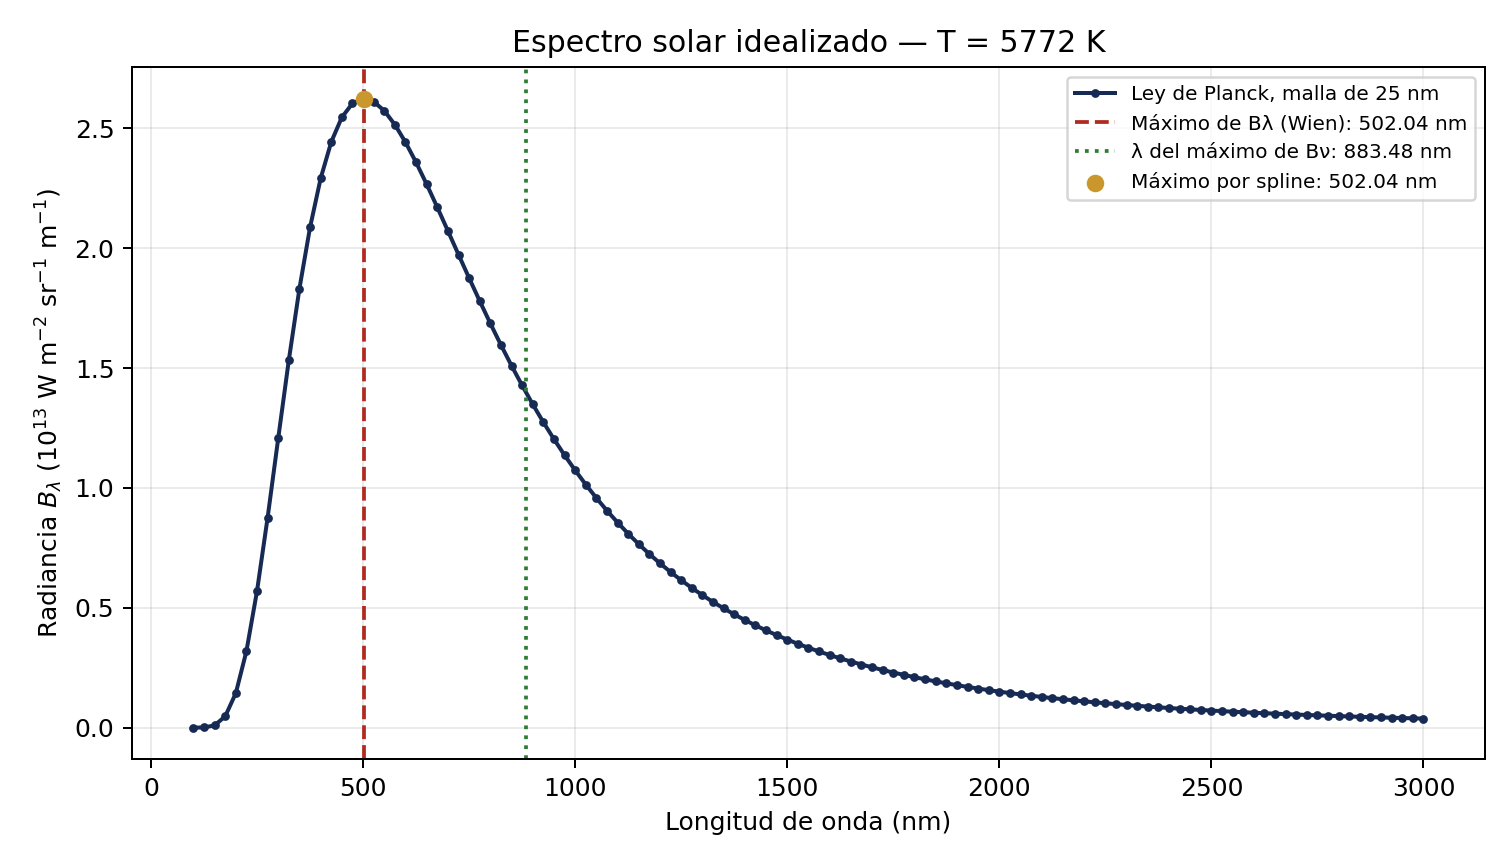
\includegraphics[width=\linewidth]{espectro_solar.png}
{\centering\footnotesize Espectro solar idealizado, malla de 25 nm.\par}
\end{minipage}

\textbf{4. Obstáculo y decisión de implementación.}
Al integrar $I=\int_0^\infty x^3/(e^x-1)\,dx$, Romberg en $[0,100]$ se detuvo en
$k=1$ con $I\approx1.6073\times10^{-15}$: los tres nodos ($0,50,100$) no
exploran la región de mayor contribución. La tolerancia diagonal da una falsa
convergencia. Con $x=t/(1-t)$, límites nulos del integrando en los extremos y
evaluación mediante $e^{-x}$ para evitar desbordamientos, se obtuvo
$I=6.4939394023$ en $k=10$ (1025 evaluaciones), frente a $\pi^4/15$.
Así, $\sigma=5.670374419\times10^{-8}$ W m$^{-2}$ K$^{-4}$.
Se conservó intacto el criterio de parada del Taller 7.

\textbf{5. Conclusión.}
Newton es eficiente cerca de la raíz física, pero depende del punto inicial;
la integración exige muestrear las regiones relevantes. Verificar con
referencias independientes y estudiar el refinamiento de malla reduce el
riesgo de interpretar una convergencia aparente como una solución física.

\textbf{Verificación:} 5/5 PASS sobre datos de referencia; pendiente regenerarlos en Colab con Fortran.\\
\textbf{Uso de IA:} Se utilizó como supervisor de codigo para ayudar en la optimizacion y redaccion correcta, tanto del programa como del informe.

\href{https://github.com/cardenascristian-web/fisica-computacional-2026ii/tree/main/Taller_8}{Repositorio: Taller 8 --- taller\_cuerpo\_negro}
\end{document}
